\documentclass[aspectratio=169]{beamer}
\usepackage[utf8]{inputenc}
\usepackage{xcolor}
\usepackage[ngerman]{babel}
\usepackage{siunitx}
\usepackage[european]{circuitikz}
\usepackage{pgfplots}
\usepackage{pdfpcnotes}
\usepackage{listings}

\usetheme{CambridgeUS}

\definecolor{toolboxOrange}{HTML}{f14531}

\setbeamercolor{section in toc}{fg=black,bg=white}
\setbeamercolor{alerted text}{fg=toolboxOrange}
\setbeamercolor*{palette primary}{fg=toolboxOrange,bg=gray!30!white}
\setbeamercolor*{palette secondary}{fg=toolboxOrange,bg=gray!15!white}
\setbeamercolor*{palette tertiary}{bg=toolboxOrange,fg=gray!10!white}
\setbeamercolor*{palette quaternary}{fg=toolboxOrange,bg=gray!5!white}
\setbeamercolor*{sidebar}{fg=toolboxOrange,bg=gray!15!white}
\setbeamercolor*{palette sidebar primary}{fg=toolboxOrange}
\setbeamercolor*{palette sidebar secondary}{fg=white}
\setbeamercolor*{palette sidebar tertiary}{fg=toolboxOrange}
\setbeamercolor*{palette sidebar quaternary}{fg=gray!10!white}
\setbeamercolor{titlelike}{parent=palette primary,fg=toolboxOrange}
\setbeamercolor{frametitle}{bg=gray!10!white}
\setbeamercolor{frametitle right}{bg=gray!60!white}

\pgfplotsset{ticks=none}

\pgfplotsset{every axis x label/.style={
  at={(0.5,0)},
  below,
  yshift=-5pt
  }
}

\pgfplotsset{every axis y label/.style={
  at={(0,0.5)},
  xshift=-15pt,
  rotate=90
  }
}

\pgfplotsset{compat=1.15}

\title{Eine Einführung in Ansible und OpenStack}

\author{L3D \& Matt}

\institute[Toolbox Bodensee]

\date{Tag der offenen Tür \the\year}

\subject{CYBER}

\logo{
\includegraphics[height=0.13\textheight]{toolbox_logo_orange}}



\begin{document}

\begin{frame}
  \titlepage
\end{frame}

\section{Einführung} 
\begin{frame}{Was ist Ansible?}
    \begin{columns}
        \begin{column}{0.4\textwidth}
            \begin{itemize}
                \item Open Source
                \item in Python geschrieben
                \item sehr gut Dokumentiert
                \item es gibt viele Beispiele
            \end{itemize}
        \end{column}
        \begin{column}{0.2\textwidth}
            
\includegraphics[width=1\textwidth]{832px-Ansible_logo.png}
        \end{column}
        \begin{column}{0.4\textwidth}
            \begin{itemize}
                \item automatisies Installieren
                \item automatisiertes Konfigurieren
                \item modularer Aufbau
                \item skaliert sehr gut
            \end{itemize}
        \end{column}
    \end{columns}
\end{frame}


\begin{frame}{Wie sieht eure IT Infrastruktur aus?}
    \begin{columns}
        \begin{column}{0.5\textwidth}
            Wer hat\ldots
                \begin{itemize}
                    \item einen Server im Internet?
                    \item einen 3D Drucker mit Octoprint?
                    \item einen Sprachassistenten eingerichtet?
                    \item einen E-Mail Server aufgesetzt? 
                \end{itemize}
        \end{column}
        \pause
        \begin{column}{0.5\textwidth}
             Dabei habt ihr bestimmt\ldots
                \begin{itemize}
                    \item Grundsystem per Hand installiert und Benutzer eingerichtet?
                    \item ggf.\ mit Shell Skripten einzelne Teile eingerichtet?
                    \item manuell die Konfigurationsdateien bearbeitet?
                    \item euer laufendes System zerschossen?
                \end{itemize}
        \end{column}
    \end{columns}
\end{frame}

  
\section{Ansible} 
\begin{frame}{Wieso Ansible?}
    \begin{columns}
        \begin{column}{1.0\textwidth}
            \centering
            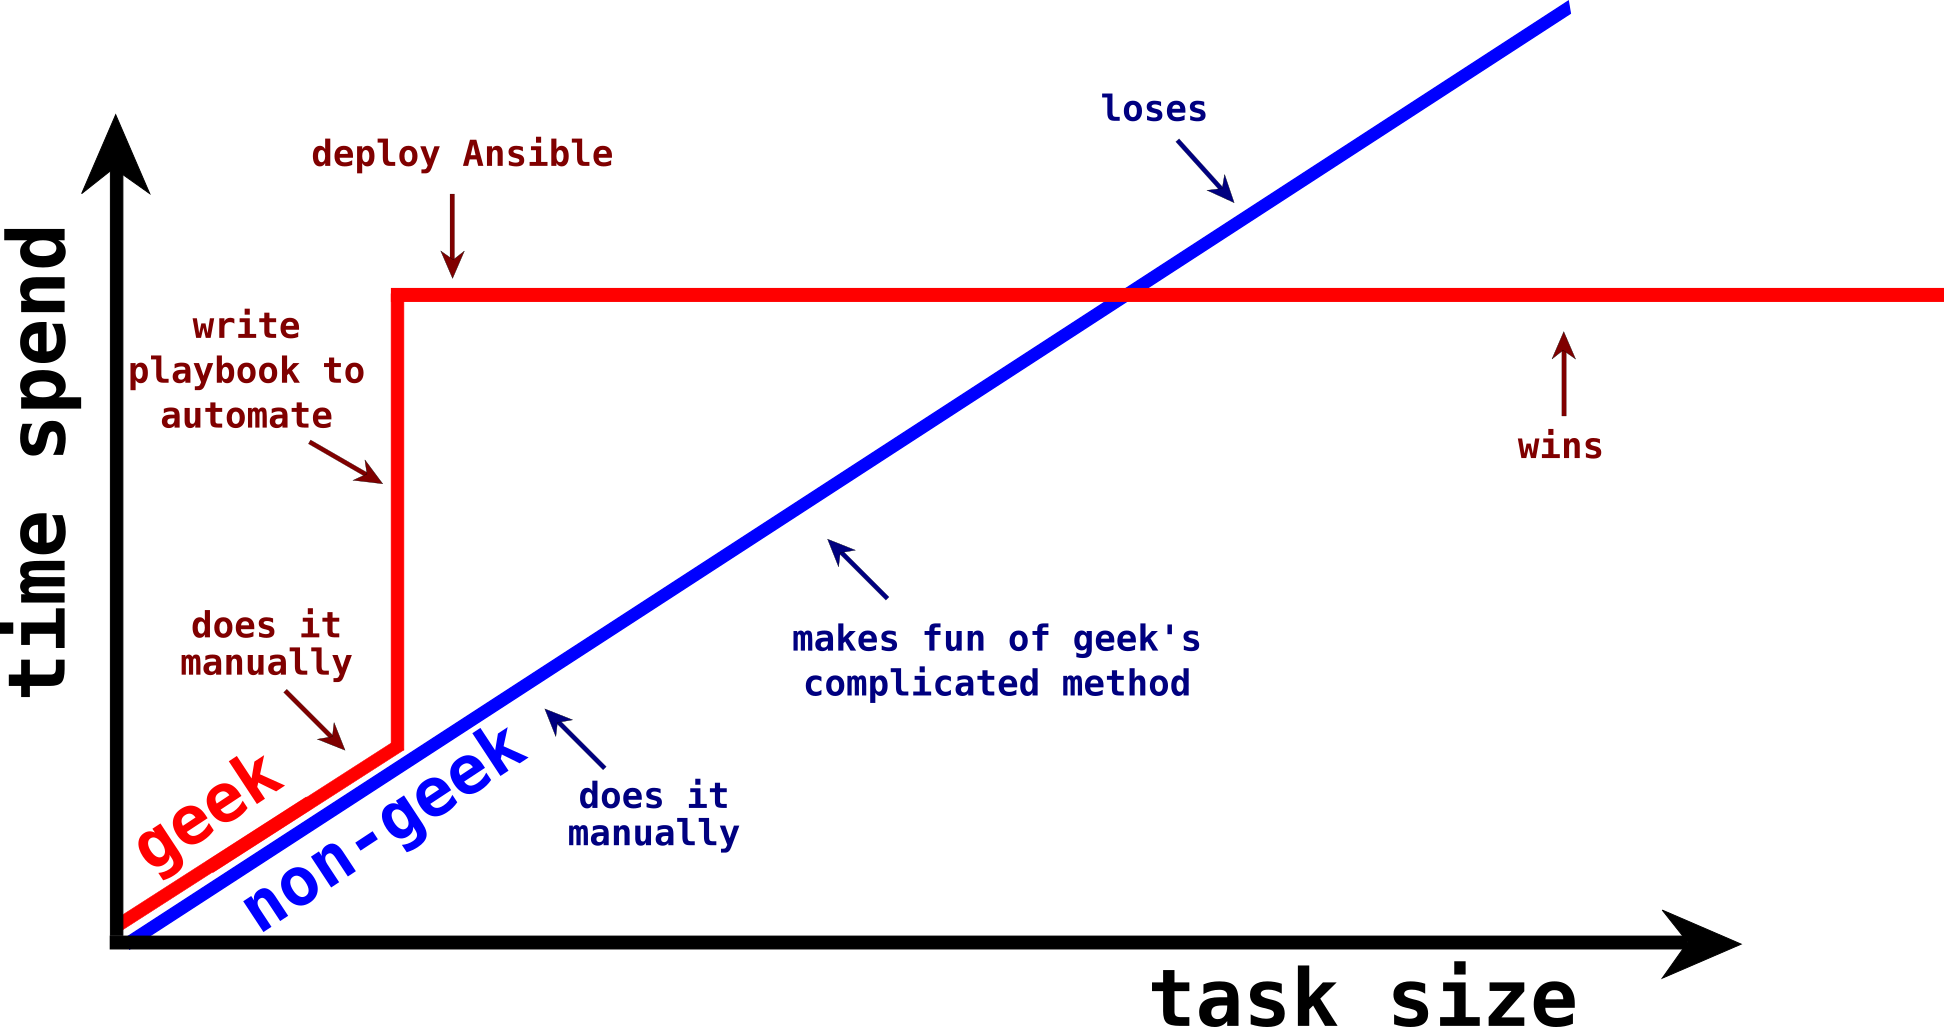
\includegraphics[width=0.85\textwidth]{why_ansible.png}
        \end{column} 
    \end{columns}
\end{frame}


\subsection{bestandteile} 
\begin{frame}{Kernbestandteile bei Ansible}
    \begin{columns}
        \begin{column}{0.33\textwidth}
            \textbf{Inventory}
            \begin{itemize}
                \item beschreibt das Inventar
                \item Hosts und Host-Gruppen
                \item globale variabeln
                \item Gruppen, Host, OS spezifische variabeln
            \end{itemize}
        \end{column}
        \pause
        \begin{column}{0.33\textwidth}
            \textbf{Modules}
            \begin{itemize}
                \item stellen funktionen zur verfügung
                \item können system resources verwalten
                \item Services, Packete, Dateien\ldots (anything really)
                \item System Befehle ausführen
                \item nicht nur auf Linux
            \end{itemize}
        \end{column}
        \pause
        \begin{column}{0.34\textwidth}
            \textbf{Playbooks}
            \begin{itemize}
                \item führen Aktionen auf der Infrastruktur aus
                \item automatisies Installieren
                \item automatisiertes Konfigurieren
                \item modularer Aufbau
                \item „like a to-do list for Ansible“
            \end{itemize}
        \end{column}
    \end{columns}
\end{frame}




\section{Freifunk} 
\begin{frame}{Bei Freifunk Bodensee werden die Server mit Ansible administriert}
    \begin{columns}
        \begin{column}{1.0\textwidth}
            \centering
            \textbf{https://github.com/ffbsee/ansible} \\
            
\includegraphics[width=0.5\textwidth]{ffbsee.png}
        \end{column}
    \end{columns}
\end{frame}

\subsection{Playbook \ldots} 
\begin{frame}{Bei Freifunk Bodensee werden die Server mit Ansible administriert}
    \begin{columns}
        \begin{column}{1.0\textwidth}
            \centering
            \textbf{https://github.com/ffbsee/ansible} \\
        \lstinputlisting[language=Python]{update_admins.yml}
        \end{column}
    \end{columns}
\end{frame}

\subsection{Ansible Hosts} 
\begin{frame}{Bei Freifunk Bodensee werden die Server mit Ansible administriert}
    \begin{columns}
        \begin{column}{1.0\textwidth}
            \centering
            \textbf{https://github.com/ffbsee/ansible} \\
        \lstinputlisting[language=Python]{hosts}
        \end{column}
    \end{columns}
\end{frame}

\subsection{Modules} 
\begin{frame}{Bei Freifunk Bodensee werden die Server mit Ansible administriert}
    \begin{columns}
        \begin{column}{1.0\textwidth}
            \centering
            \textbf{https://github.com/ffbsee/ansible} \\
            \lstinputlisting[language=Python]{update.yml}
        \end{column}
    \end{columns}
\end{frame}




\section{Openstack} 
\begin{frame}{Openstack}
    \begin{columns}
        \begin{column}{1.0\textwidth}
            \centering
            
\includegraphics[width=0.5\textwidth]{openstack.png}
        \end{column}
    \end{columns}
\end{frame}



\section{Ende}
 \subsection{}
\begin{frame}{}
    \begin{center}
        {\Huge Vielen Dank für eure Aufmerksamkeit!}
        
        \vspace{0.8cm}
        
        {\huge Gibt es noch Fragen?}
    \end{center}
\end{frame}

\end{document}
